\documentclass[10pt, a4paper, twoside]{article}

% Set up the standard margins for the document
% 42.2 left & 15.5 right is same as Forsling, Neymark
% 21.3 top  & 20 bottom is same as Olofsson
\usepackage[left=19.5mm, right=19.5mm, top=21.3mm, bottom=20mm]{geometry}

\usepackage{subcaption}
\usepackage{float}

% Input file character encoding (kinda useless if we don't
% use åäö and stuff, but it doesn't hurt to have it)
\usepackage[utf8]{inputenc}
%\usepackage[swedish]{babel}

% Block Comments
\usepackage{comment}

% No indentation in new paragraph
\usepackage{parskip}

% To include graphics
\usepackage{graphicx}

% More mathematical symbols and fonts
\usepackage{amsmath}
\usepackage{amsfonts}
\usepackage{amssymb}

% Simple list
\usepackage[ampersand]{easylist}
\ListProperties(Hide=100, Hang=true, Progressive=5ex, Style*=$\bullet$ ,
Style2*=-- ,Style3*=$\circ$ ,Style4*=\tiny$\blacksquare$ )


% Clickable internal links
\usepackage{hyperref}
\usepackage[all]{hypcap} % without this the link takes you to the caption, not the top of the image
\hypersetup{ % Settings for links in documnet
	setpagesize = false, % Don't allow hyperref to change page size. Tips från Micke Olofsson
	colorlinks = true,   % No boxes around links
	linkcolor = black,citecolor = black,filecolor = black,urlcolor = black, % don't color links
}

% To include to first page pdf file
\usepackage{pdfpages}

% Add section number to equation and figure number (ex: 5.11 instead of simply 11)
\numberwithin{equation}{subsection}
\numberwithin{figure}{section}
\numberwithin{table}{section}

% Show program code listings in document
\usepackage{listings}

%
% Header stuff
%
\usepackage{fancyhdr}
\setlength{\headheight}{15pt}

\fancyhf{}
\fancyhead[LE, RO]{\thepage}
\fancyhead[RE]{TSBB15 2013: Project Report}
\fancyhead[LO]{Object Tracking in Image Sequences}

\fancypagestyle{plain}{ %
\fancyhf{} % remove everything
\renewcommand{\headrulewidth}{0pt} % remove lines as well
\renewcommand{\footrulewidth}{0pt}}
%
% End header stuff
%




\begin{document}

% First page

\includepdf{Cover/cover.pdf}


% Project identity page
\newpage
\pagestyle{fancy}
\pagenumbering{roman}
\setcounter{page}{2} % sets the current page number to 2 

\begin{center}
    \vspace*{4\baselineskip}

	\textbf{\huge Project Kitchen Occupation} \\
	\vspace*{0.5\baselineskip}
	Bilder och Grafik CDIO, HT 2013 \\
	Department of Electrical Engineering (ISY), Link\"{o}ping University
	
	\vspace*{2\baselineskip}
	\textbf{\LARGE Participants}


	{\footnotesize 
	\begin{tabular}{|p{2.7cm}|p{1cm}|p{5cm}|p{2cm}|p{3.4cm}|}
		\hline
		\textbf{Name} & \textbf{Tag} & \textbf{Responsibilities} & \textbf{Phone} & \textbf{E-mail} \\
		\hline
		Mattias Tiger & MT & Project manager & 073--695\,71\,53 & matti166@student.liu.se \\
		\hline
		Erik Fall & EF & -- & 076--186\,98\,84 & erifa226@student.liu.se \\
		\hline
		Gustav Häger & GH & System integration & 070--649\,03\,97 & gusha124@student.liu.se \\
		\hline
		Malin Rudin & MR & -- & 073--800\,35\,77 & malru103@student.liu.se \\
		\hline
		Alexander Sjöholm & AS & -- & 076--225\,11\,74 & alesj050@student.liu.se \\
		\hline
		Martin Svensson & MS & Documentation & 070--289\,01\,49 & marsv106@student.liu.se \\
		\hline
		Nikolaus West & NW & Testing & 073--698\,92\,60 & nikwe491@student.liu.se \\
		\hline
	\end{tabular}
	}

{\footnotesize 
\vspace{0.5\baselineskip}
\textbf{Homepage}: TBA \\
\vspace{1\baselineskip}

\textbf{Customer}: Joakim Nejdeby, Link\"{o}ping University, Origo 3154 \\
\textbf{Customer contact}: 013--28\,17\,57, joakim.nejdeby@liu.se \\
\textbf{Project supervisor}: Fahad Khan, Link\"{o}ping University, fahad.khan@liu.se \\
\textbf{Examiner}: Michael Felsberg, michael.felsberg@liu.se \\
}

\end{center}



% table of contents
\newpage
\tableofcontents
\listoffigures
\listoftables

% list of figures
%\newpage
%\listoffigures


% Document history page
\newpage
\vspace*{5\baselineskip}

\begin{center}
\textbf{\LARGE Document history}

{ \footnotesize 
\begin{tabular}{|p{1cm}|p{2.0cm}|p{5cm}|p{1.5cm}|p{2cm}|}
	\hline

	\textbf{Version} & \textbf{Date} & \textbf{Changes} & \textbf{Sign} & \textbf{Reviewed} \\
	
	\hline
	0.1 & 2013--12--13 & Initial draft & MS & MT\\
	
	\hline
	 &  &  &  &  \\
	
	\hline
\end{tabular}
}
\end{center}


% Blank page
%\newpage
%\thispagestyle{empty}
%\mbox{}



%
% Content start
%
\newpage
\pagenumbering{arabic}

\newpage
\section{Introduction}
\label{sec:introduction}
What to write here? maybe nothing.

\subsection{About this document}
This docment, is the user manueal....


\newpage
\section{System Overview}
\label{sec:system_overview}
Below is an overview of the entire system. Data collection from several rooms are performed simultaneously, and processed data is presented to the user through a web page.

\vspace{0.5cm}
\begin{figure}[htb]
	\centering
	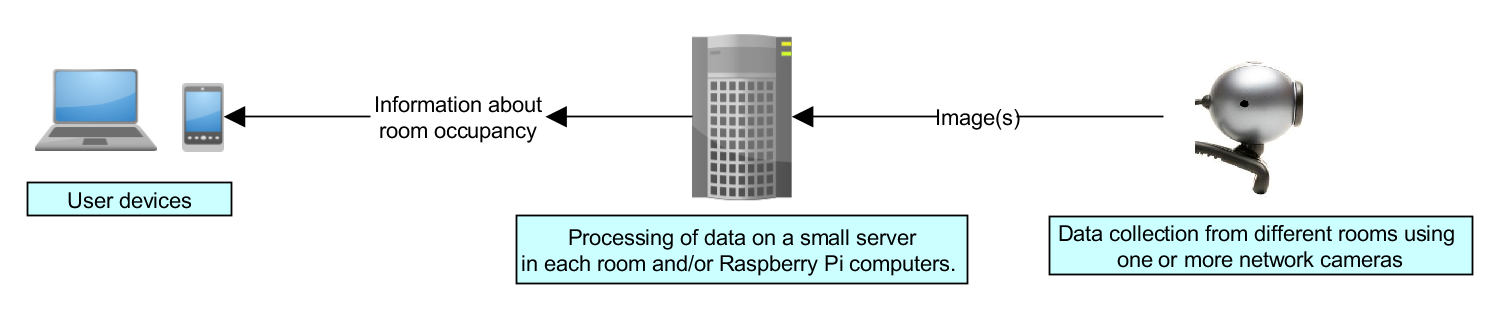
\includegraphics[width=170mm]{images/system_overview.png}
	\caption[System overview]{\textit{A simplified overview of the system}}
	\label{fig:block_overview2_fig}  %Skapar referens till figuren
\end{figure}

\subsection{Rough description of the system}
The camera(s) used to collect data are connected to a local network via Ethernet cables. The main program collects data from the cameras in a room to perform an estimation of room usage intensity, which is then presented to the user in an understandable format, e.g. estimated waiting time.

\subsection{Components}
The main components of the system is of course the cameras, as well as the software running on the central server.

\subsubsection{Hardware}
The cameras are network cameras powered via Ethernet cable, mounted in way that allows for good performance and low installation costs. The hardware is described more thoroughly on this in section \ref{sec:hardware}.

\subsubsection{Software}
The software will be running on a central server, where both image processing and estimation of queue size and waiting time takes place. For a more thorough description of the image processing and estimation programs, see section \ref{sec:software}.

\subsection{Usability and installation}
In order to create a system that is cheap to use and install, it needs to be easy to set up, which is why a user's manual and an installation/calibration program is provided with the system if necessary. As for the usability, relevant data is presented to the user on a web page (see section \ref{sec:usage}). 



\newpage
\section{Current pipeline}
\label{sec:current_pipeline}
This section describes the image processing pipeline that is delivered with the system and that has yielded the best performance so far. Some less successful attempts are described in appendices \ref{sec:bg_subtraction}, \ref{sec:hough_circles}, and \ref{sec:stereoBM}. 

\subsection{Sensors}
After reading several papers on counting people using a single camera with top-down view, and implementing the methods described in said papers, the realization was made that, in order to be able to solve the problem described in section \ref{sec:introduction}, some form of depth information would be necessary. Both stereo and Kinect-style sensors were considered. However due to time limitations and a customer desire to run the system on cheap hardware, the Microsoft Kinect sensor was chosen.

\subsection{Image processing}
The human segmentation is based on the assumption that human heads are distinguishable modes in the depth image and that people moving very close to each other seldom differ much more than a head in height. It is realized by a series of threshold and morphological operations, contour drawing and searches for local maxima. The output from some of the steps in the segmentation algorithm can be seen in figure \ref{fig:image_processing_steps}.

\begin{figure}[htb]
	\centering
	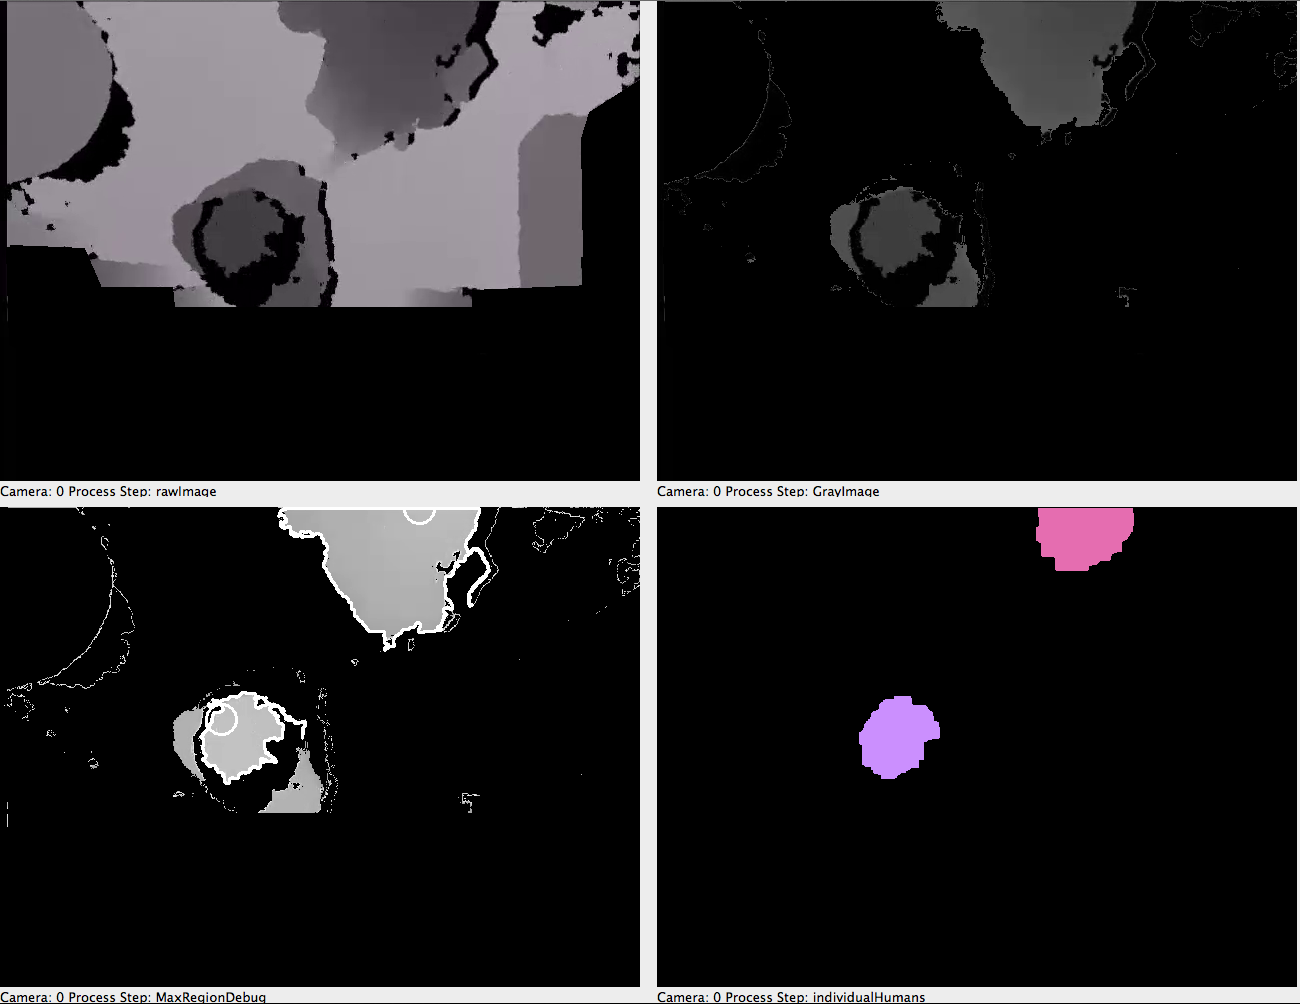
\includegraphics[width=\linewidth]{images/image_processing_steps.png}
	\caption[Image processing steps]{\textit{Image processing steps. The figure shows the results from four of the processing steps in the image processing pipeline.\\
		Top left: Raw depth image.\\ 
		Top right: Image after first threshold operation.\\ 
		Bottom left: Contour drawing and local maxima detection.\\ 
		Bottom right: Segmented human heads.}}
	\label{fig:image_processing_steps}  %Skapar referens till figuren
\end{figure}

\newpage
\subsection{Tracking and counting}
The tracking algorithm performs six different steps for each frame iteration. The tracker has a list objects found by earlier image processing steps and one list of objects passed from the previous frame. Tracking is done by pairing closest objects with each other, from previous frame to the current frame. Objects need to live for a predetermine configurable amount of frames before it will be counted. This will prevent false flickering objects from generating false entries. Lost objects are also kept alive for some frames, this enables objects to be lost and found. Figure \ref{fig:trackingexample} illustrates how objects are seen as real objects, lost objects or potential objects, depending on their lifetime. 

\begin{figure}[htb]
	\centering
	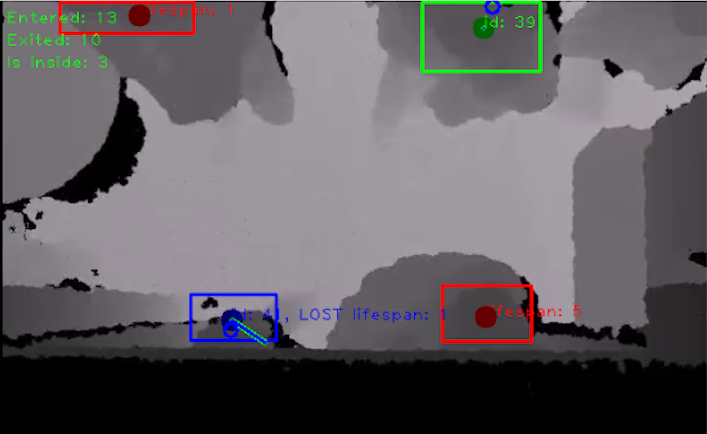
\includegraphics[width=0.7\linewidth]{images/trackingexample2.png}
	\caption[Entry exit circles]{\textit{Visualization of the tracking. The image shows one person (green box) who has lived long enough to be considered a person, two (red boxes) who has just been found and one (blue box) which is a person who’s just been lost}}
	\label{fig:trackingexample}  %Skapar referens till figuren
\end{figure}


To register if objects enter or exit the room the objects has to fulfill some requirements. To be considered as entered, an object has to be found in a door area and pass three circle lines in addition to have existed a minimum of a set amount of frames. To be registered as exited an object has to have existed a minimum of a set amount of frames and disappear inside a door area, while also at least once passed the three lines. Examples of these circle lines and a door area can be seen in figure \ref{fig:entry_exit}.

\begin{figure}[htb]
	\centering
	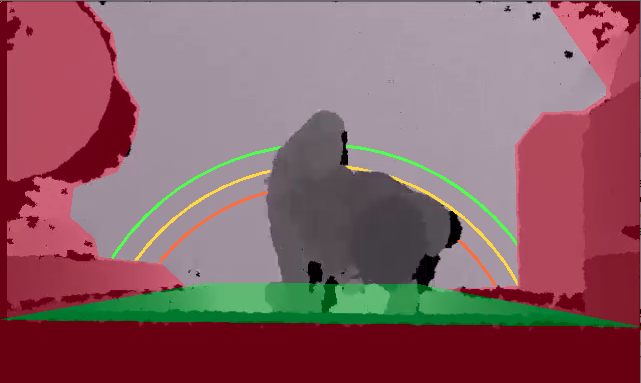
\includegraphics[width=0.7\linewidth]{images/entryexitexample.png}
	\caption[Entry exit circles]{\textit{Entry and exit counting. Three circles are used to decide when a person has entered. The green area is the door area and the red area is excluded by the system.}}
	\label{fig:entry_exit}  %Skapar referens till figuren
\end{figure}

\newpage

\subsection{Queue severity estimation}
Queues are detected by using the positions and velocities, which are calculated using a simple Kalman filter, of all visible persons. This information is used to draw splines between each of the visible persons. Two people are then considered to be in a queue if a short enough spline can be drawn between them. The result is that persons that stand still or move slowly along the same path are considered to be in a queue. Examples of this can be seen in \ref{fig:visible_queue} and \ref{fig:no_queue}.
\\ \\
Queue severity is estimated by considering the proportion of frames with visible queues, and optionally the amount of people inside the room, over a set time interval. 
\begin{figure}[H]
\centering
\begin{subfigure}{.5\textwidth}
  \centering
  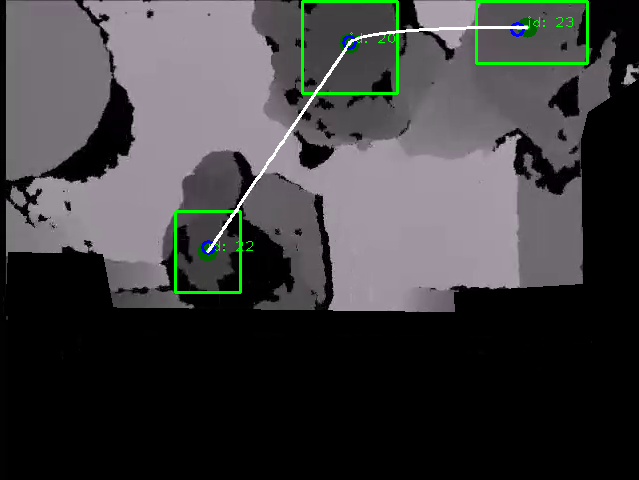
\includegraphics[width=0.9\linewidth]{images/visibleQueue.png}
  \caption{When persons are close together and moving slowly, \\
  			 they are connected by short splines and thus considered\\
  			  to be in a queue.}
  \label{fig:visible_queue}
\end{subfigure}%
\begin{subfigure}{.5\textwidth}
  \centering
  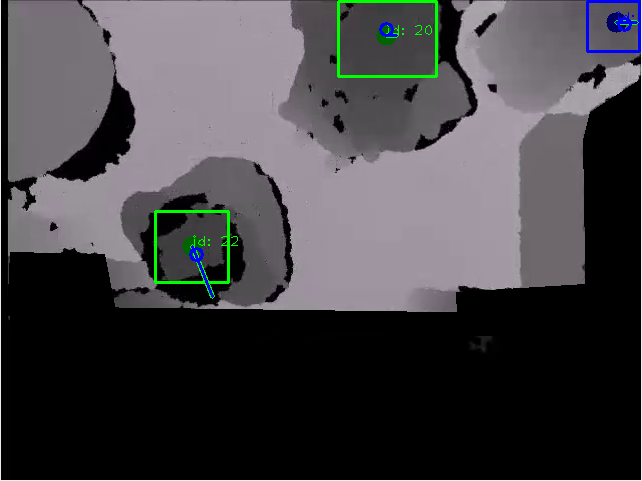
\includegraphics[width=0.9\linewidth]{images/noQueue.png}
  \caption{Persons moving in different directions, with large velocity, are connected by longer splines, and are thus not considered to be in a queue.}
  \label{fig:no_queue}
\end{subfigure}
\caption[Queue detection]{\textit{Detection of queues using splines. The images show the result of the queue detection steps in two different cases.}}
\label{fig:queue_detection}
\end{figure}





\newpage
\section{System Evaluation}
\label{sec:evaluation}
In order to measure performance a performance metric needs to be defined, and test data and training data needs to be collected from several system use cases. The number of people entering and exiting is thoroughly evaluated according to the below described criteria. However, because the queue severity estimation is poorly defined, this part of the system has only been visually inspected to ensure reasonable results. The system also includes functionality to evaluate the tracking, which is not currently used but is further explained in appendix \ref{sec:tracker_evaluation}.

\subsection{Ground Truth}
The evaluation needs access to ground truth data, which defines the best possible achievable counter output. Currently the ground truth files consist of arrays with values for each frame denoting how many people entered or exited in that specific frame. Since the focus of the system lies on maintaining a correct count over some time, the exact moment when a person exits the room is deemphasized.

\subsection{Evaluation Metric}
Reading several papers on the subject of people counting it became clear that no standard for measuring people counting performance exists. In the absence of such a standard the below measurement methods were chosen since they are thought to provide an accuracy measurement of the outputs the customer is most likely to be interested in (total number of people using the room, and total number of people currently in the room).
What was decided to be most desirable and important to measure was the number of people entering, leaving, and the error in the room occupancy estimation as a function of the total number of people that have entered or left the room. The equations for the three different metrics are defined below, where the subscript \textit{Est} denotes the value generated by the system and \textit{GT} the true value that was read from the ground truth data.

\begin{equation}
\label{eq:in_accuracy}
A_{in} = 1 - \Big{\lvert}\frac{\sum_{frames}{in_{Est}}-\sum_{frames}{in_{GT}}}{\sum_{frames}in_{GT}}\Big{\rvert}
\end{equation} 

\begin{equation}
\label{eq:out_accuracy}
A_{out} = 1 - \Big{\lvert}\frac{\sum_{frames}{out_{Est}}-\sum_{frames}out_{GT}}{\sum_{frames}out_{GT}}\Big{\rvert} 
\end{equation} 

\begin{equation}
\label{eq:occupancy_bias}
A_{bias} = \frac{(\sum_{frames}{in_{Est}-\sum_{frames}out_{Est}})-(\sum_{frames}{in_{GT}-\sum_{frames}out_{GT}})}{\sum_{frames}in_{GT}+out_{GT}} 
\end{equation} 






\newpage
\section{Results}
\label{sec:results}
The system results were obtained by evaluating against three recorded sequences from three different kitchens. The sequences were labeled manually using a self-developed labeling program.

\subsection{Evaluation Scores}
In table \ref{tab:evaluation_performance} below the video clips chosen for the evaluation are presented, along with the achieved accuracy measurements. The first 5 minutes of the data set R-Kitchen was used when tuning and developing the system. The data set B25-Kitchen show how robust our system is, since the system wasn't calibrated for the specific room and the camera was slightly miss-placed. The majority of the errors was confirmed to depend on these two factors by ocular inspection.

\begin{table}[h]
\centering
	\begin{tabular}{r | c | c | c | c | c  }
			\emph{Sequence Name}		&  Total entered (GT) & \emph{$A_{in}$} & Total exited (GT) & \emph{$A_{out}$} & length \\
			\hline \hline
			R-Kitchen			& 108 (108) people & 99 \% & 101 (104) people & 97 \% & 32 min\\
			U-Kitchen			& 123 (122) people & 99 \% & 134 (135) people & 99 \% & 31 min  \\
			B25-Kitchen			& 131 (141) people & 93 \% & 82 (91) people & 90 \% & 30 min \\
			\end{tabular}
	\caption[System performance]{\textit{Counting performance according to the evaluation metric as described in section \ref{sec:evaluation}.}}
	\label{tab:evaluation_performance}
\end{table}

Plots of ground truth comparison and accuracy for the evaluation sequences can be found in figure \ref{fig:R-kitchen entries}, \ref{fig:R-kitchen exits}, \ref{fig:B25-kitchen entries} and \ref{fig:B25-kitchen exits}.

\begin{figure}[H]
\centering
\begin{subfigure}{.5\textwidth}
  \centering
  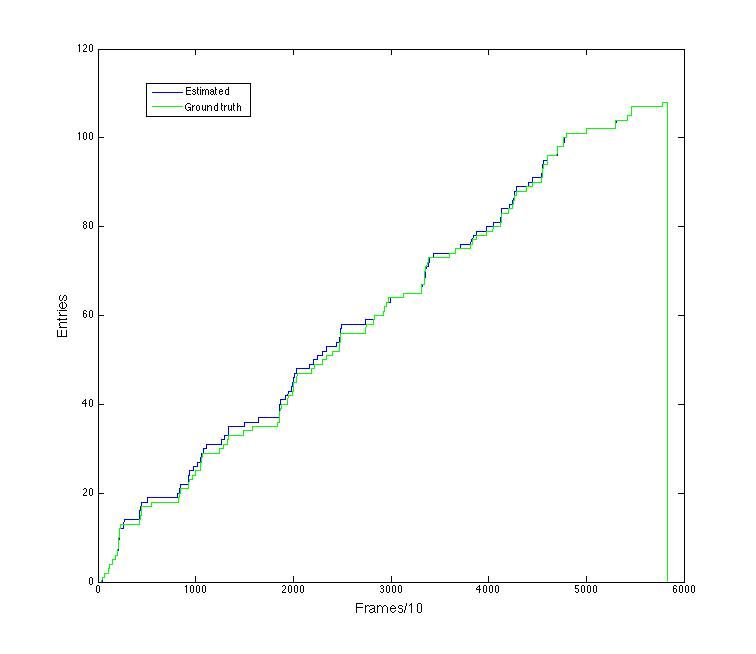
\includegraphics[width=1.1\linewidth]{images/EntriesTest.png}
  \caption{Measured entries and ground truth}
  \label{fig:sub1}
\end{subfigure}%
\begin{subfigure}{.5\textwidth}
  \centering
  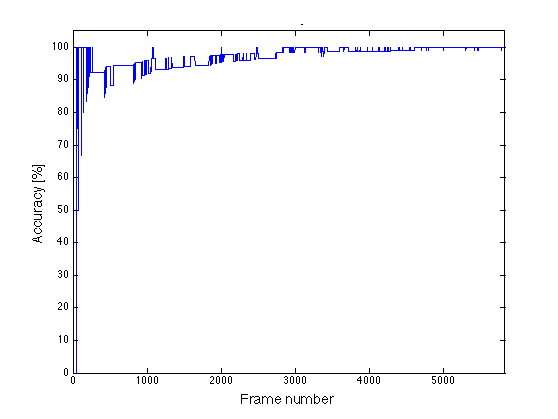
\includegraphics[width=1.1\linewidth]{images/AccEntriesTest.png}
  \caption{Accuracy}
  \label{fig:sub2}
\end{subfigure}
\caption[R-kitchen entries]{\textit{R-Kitchen data. Plot of measured entries, ground truth and accuracy}}
\label{fig:R-kitchen entries}
\end{figure}
\newpage

\begin{figure}[H]
\centering
\begin{subfigure}{.5\textwidth}
  \centering
  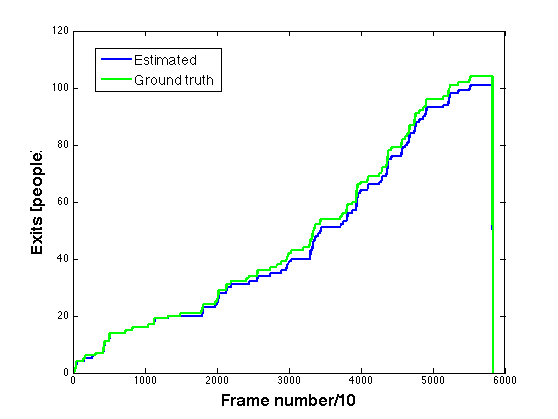
\includegraphics[width=1.1\linewidth]{images/ExitsTest.png}
  \caption{Measured exits and ground truth}
  \label{fig:sub1}
\end{subfigure}%
\begin{subfigure}{.5\textwidth}
  \centering
  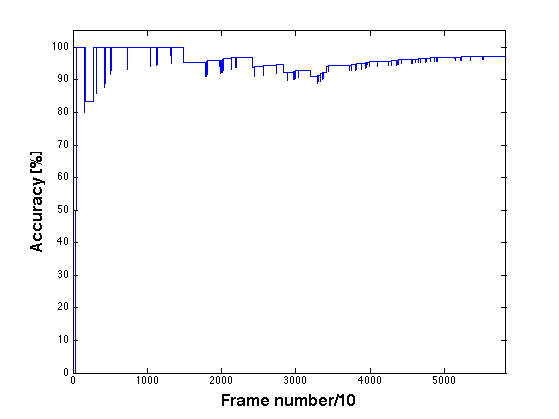
\includegraphics[width=1.1\linewidth]{images/AccExitsTest.png}
  \caption{Accuracy}
  \label{fig:sub2}
\end{subfigure}
\caption[R-kitchen exits]{\textit{R-Kitchen data. Plot of measured exits, ground truth and accuracy}}
\label{fig:R-kitchen exits}
\end{figure}


\begin{figure}[H]
\centering
\begin{subfigure}{.5\textwidth}
  \centering
  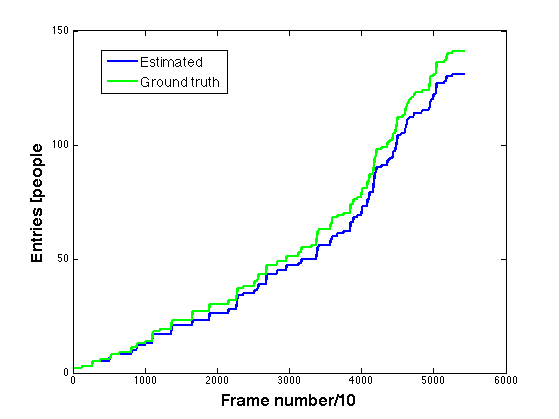
\includegraphics[width=1.1\linewidth]{images/entriesGTB25.png}
  \caption{Measured entries and ground truth}
  \label{fig:sub1}
\end{subfigure}%
\begin{subfigure}{.5\textwidth}
  \centering
  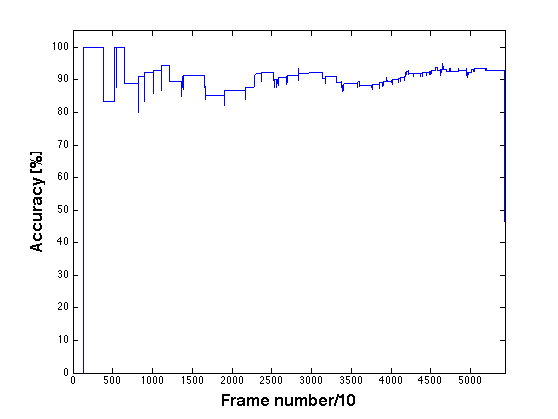
\includegraphics[width=1.1\linewidth]{images/accInB25.png}
  \caption{Accuracy}
  \label{fig:sub2}
\end{subfigure}
\caption[B25-kitchen entries]{\textit{B25-Kitchen data. Plot of measured entries, ground truth and accuracy}}
\label{fig:B25-kitchen entries}
\end{figure}

\begin{figure}[H]
\centering
\begin{subfigure}{.5\textwidth}
  \centering
  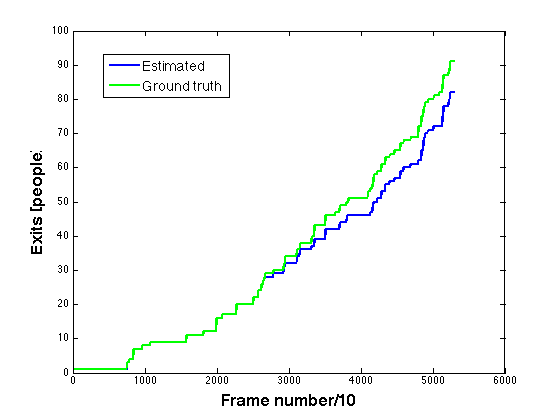
\includegraphics[width=1.1\linewidth]{images/exitsGTB25.png}
  \caption{Measured exits and ground truth}
  \label{fig:sub1}
\end{subfigure}%
\begin{subfigure}{.5\textwidth}
  \centering
  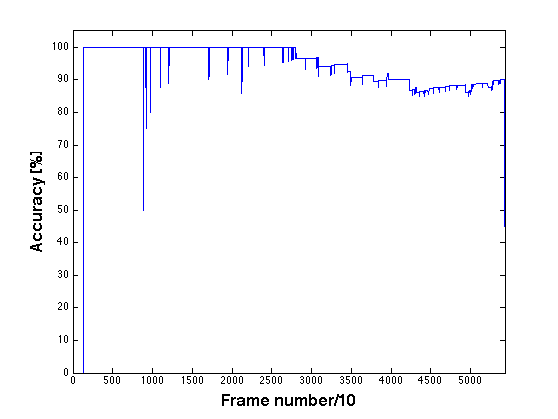
\includegraphics[width=1.1\linewidth]{images/accOutB25.png}
  \caption{Accuracy}
  \label{fig:sub2}
\end{subfigure}
\caption[B25-kitchen exits]{\textit{B25-Kitchen data. Plot of measured exits, ground truth and accuracy}}
\label{fig:B25-kitchen exits}
\end{figure}

\begin{figure}[H]
\centering
\begin{subfigure}{.5\textwidth}
  \centering
  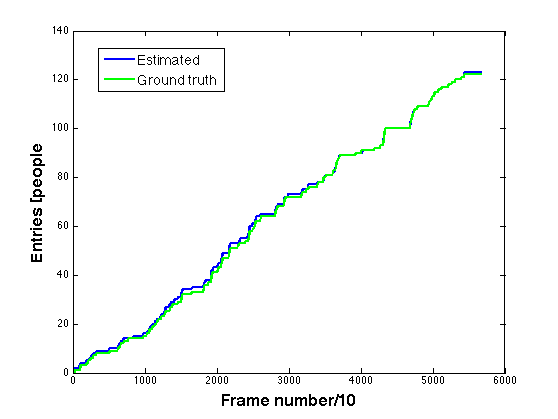
\includegraphics[width=1.1\linewidth]{images/entriesGTU.png}
  \caption{Measured entries and ground truth}
  \label{fig:sub1}
\end{subfigure}%
\begin{subfigure}{.5\textwidth}
  \centering
  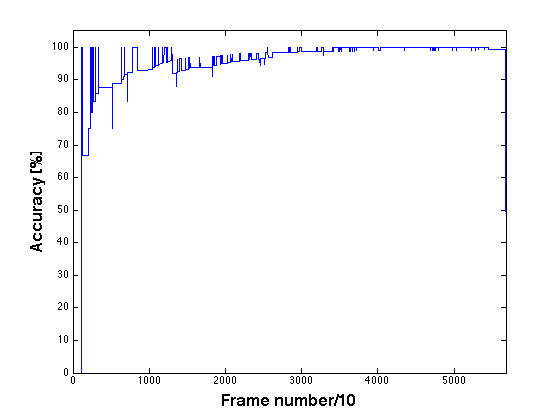
\includegraphics[width=1.1\linewidth]{images/accInU.png}
  \caption{Accuracy}
  \label{fig:sub2}
\end{subfigure}
\caption[B25-kitchen entries]{\textit{U-Kitchen data. Plot of measured entries, ground truth and accuracy}}
\label{fig:B25-kitchen entries}
\end{figure}

\begin{figure}[H]
\centering
\begin{subfigure}{.5\textwidth}
  \centering
  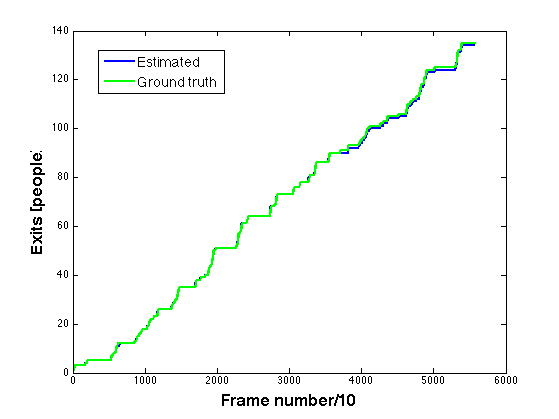
\includegraphics[width=1.1\linewidth]{images/exitsGTU.png}
  \caption{Measured exits and ground truth}
  \label{fig:sub1}
\end{subfigure}%
\begin{subfigure}{.5\textwidth}
  \centering
  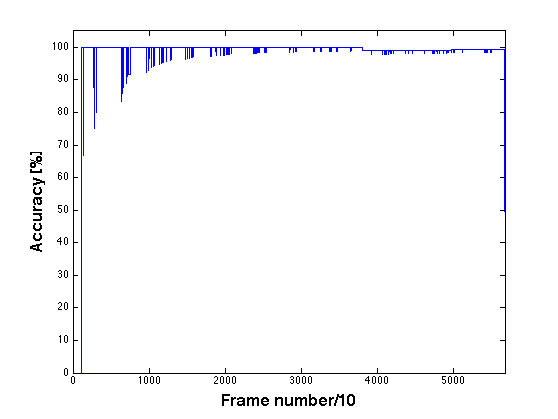
\includegraphics[width=1.1\linewidth]{images/accOutU.png}
  \caption{Accuracy}
  \label{fig:sub2}
\end{subfigure}
\caption[B25-kitchen exits]{\textit{U-Kitchen data. Plot of measured exits, ground truth and accuracy}}
\label{fig:B25-kitchen exits}
\end{figure}

\subsection{Queue Detection}
Below in figure \ref{fig:Queue Detection}, several screenshots from the queue detection steps are shown. Several difficult cases are shown to be handled gracefully. The main difficulty is when the small field of view gives situations where a queue is present but only one queuing person is detected at one time. However, this is usually handled well by the queue severity estimation, as the thresholds for the proportion of frames with detected queues can be calibrated to account for these results, given that several queuing persons are in view at simultaneously sometimes. 

\begin{figure}[H]
\centering
\begin{subfigure}{.4\textwidth}
  \centering
  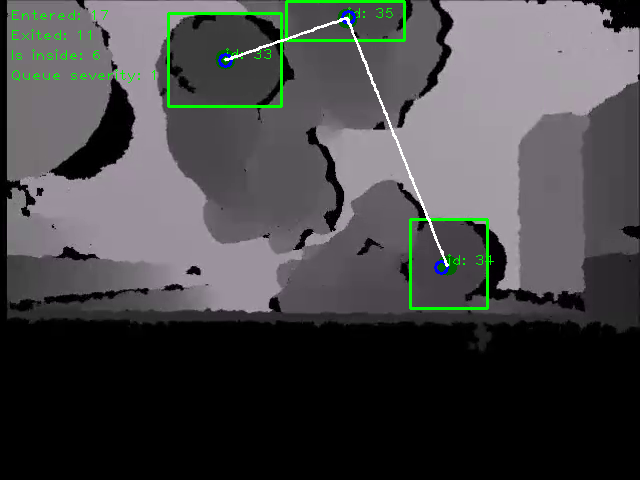
\includegraphics[width=1.0\linewidth]{images/queueDetected3.png}
  \caption{A queue of stationary persons is detected.}
  \label{fig:sub1}
\end{subfigure}
\begin{subfigure}{.4\textwidth}
  \centering
  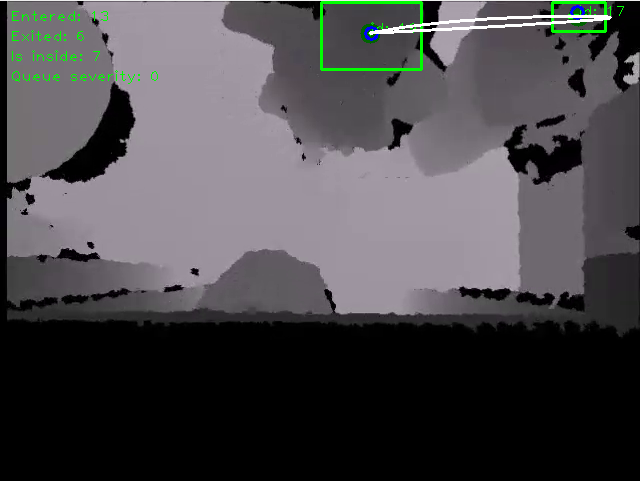
\includegraphics[width=1.0\linewidth]{images/queueDetected1.png}
  \caption{A queue is detected with unsure direction.}
  \label{fig:sub2}
\end{subfigure} 
\begin{subfigure}{.4\textwidth}
  \centering
  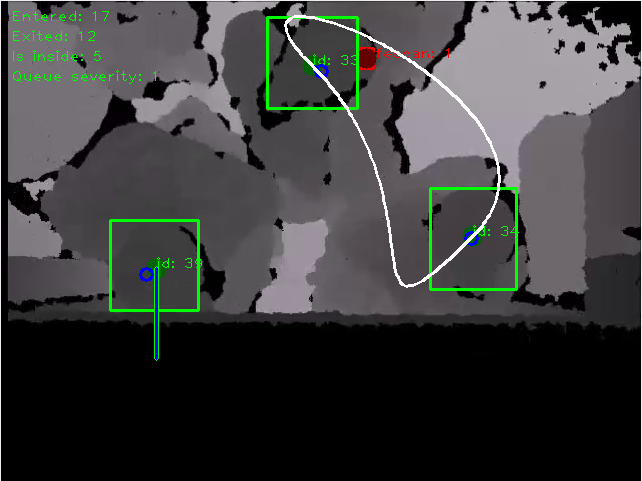
\includegraphics[width=1.0\linewidth]{images/queueDetected2.png}
  \caption{The individuals on his/her way out is not counted in the queue.}
  \label{fig:sub3}
\end{subfigure}
\begin{subfigure}{.4\textwidth}
  \centering
  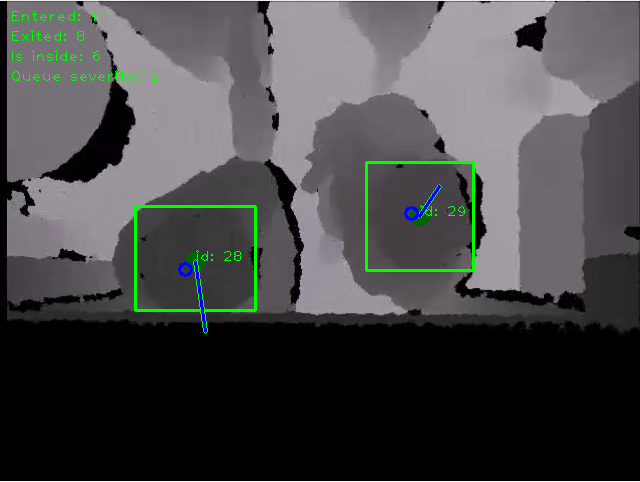
\includegraphics[width=1.0\linewidth]{images/noQueue1.png}
  \caption{Correctly, no queue is detected since both detected objects are moving in opposite directions.}
  \label{fig:sub4}
\end{subfigure}
\begin{subfigure}{.4\textwidth}
  \centering
  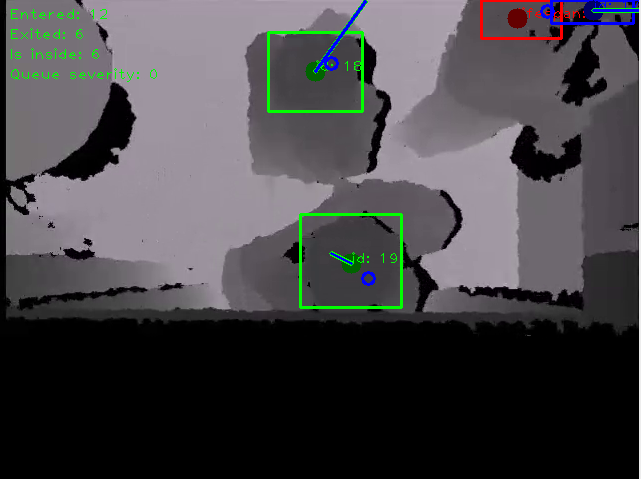
\includegraphics[width=1.0\linewidth]{images/noQueue2.png}
  \caption{Correctly, no queue is detected since both detected objects are moving too fast.}
  \label{fig:sub5}
\end{subfigure} 
\begin{subfigure}{.4\textwidth}
  \centering
  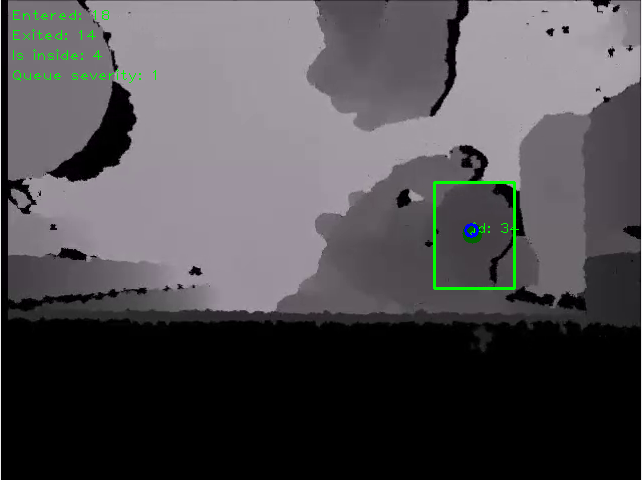
\includegraphics[width=1.0\linewidth]{images/queueNotDetected.png}
  \caption{Incorrectly, no queue is detected due to that the next person's head is not in view.}
  \label{fig:sub6}
\end{subfigure}%
\caption[Queues]{\textit{Depth data images from the R-Kitchen, with green boxes showing detected objects,blue dots showing object centers, blue lines from the centers showing estimated velocities, and white curves showing the fitted Beziér splines.}}
\label{fig:Queue Detection}
\end{figure}

\subsection{Discussion}
The performance of the R-Kitchen and U-Kitchen sets are very good. The R-Kitchen set is a sequence of 30 minutes, where only the first 5 was used for tuning. The system performed worse on the B25-Kitchen sequence, but that is probably explained by the fact that the sensor was a bit misplaced, making parts of the upper door area on one side to be outside of the field of view, as well as the lack of room-calibration. The reason no more data sets were used was simply that no more time was available.

The queue detection and severity estimation in general worked as expected but performed worse for more sparse queues, in combination with a small field of view.  




\newpage
\section{Conclusions}
\label{sec:conclusions}
The most prominent conclusion that can be drawn from this project is that the problem of counting people passing through a doorway using a single camera is much harder than what it may seem at first glance. Another is the fact that spending time on building a good software architecture increases the possibility to handle fast changes of project circumstances, as were the case here. Because of the high quality of the software architecture, we were able to change approach quickly and achieve good results in a short period of time.\\
\\


\subsection{Improvement suggestions}
As with most projects the possible improvements are many. An improvement that would most likely yield a notable increase in performance would probably be to replace the current Micorsoft Kinect with a similar sensor that has better depth accuracy. The biggest obstacle to more stable performance and to be able to give more reliable estimates of the queue severity is the small field of view afforded by the Microsoft Kinect. A solution to this could be to calculate depth from several cameras if the disparity map can be calculated fast enough on cheap hardware. Another approach might be to have one Kinect on each side of each entrance so that a larger field of view would be obtained without significant inference between the two sensors.\\
\\


















\newpage
\appendix
\addcontentsline{toc}{section}{Appendices} % Add an entry for this in the table of contents

\section{Additional functionality - Tracker accuracy evaluation.}
\label{sec:tracker_evaluation}

Previous experience of group members on implementing object tracking in video sequences sparked the idea of incorporating a method for evaluating object trackers into the system evaluation. The main reason for this was that an implementation in C++ using OpenCV was already available from a previous computer vision project. The evaluation metric available was the MOTA/MOTP system defined by Bernardin \& Stiefelhagen in (2008) \cite{MOTA}. \\

Initially the evaluation system promised good results as the implementation easily fit into the project architecture. The first evaluation was performed on short RGB test data files. Even though the implementation went smoothly, obtaining ground truth data was a whole other matter. No suitable (top-down view of people passing a doorway) clips with pre-created ground truth data were found, which meant that ground truth data would have to be labeled manually. The ground truth data was on the format specified by the CAVIAR project \cite{CAVIAR}. A program for labeling sequences frame by frame is available on the CAVIAR homepage. Because the tracker evaluation depends on accurate object positions it soon became clear that labeling enough ground truth data by stepping through sequences frame by frame to provide a feasible basis for evaluation would be far to time consuming. This is especially noticeable when one considers the fact that the actual goal of the project is to simply count people passing by, and not to track them with perfect accuracy.

The tracking evaluator is included with the final software because it works well and might be useful if the software is to be used for an other application, for example people tracking outdoors or other open spaces.

\newpage

\section{An unsuccessful attempt - people detection using background-foreground segmentation.}
\label{sec:bg_subtraction}

A very simple solution was tried early in the project. It consisted of a Mixture of Gaussian model \cite{Gardel} used for segmenting the moving foreground from the background as a binary mask. After the segmentation, all connected moving objects were found and tracked using a simple tracker. This approach was developed and performed well for tracking people moving relatively fast, but worse or not at all for people moving slow and standing still. This approached suffered from problems such as be unable to handle common occlusions when people stand and move too close to each other, especially when doing so from entering to leaving the field of view. To detect individual persons in such situations required more advanced methods, some of which were tried, but never really tuned or good enough to perform well enough. Further improvements on this approach were therefore never implemented. The approach also required quite some morphological operations to connect loosely connected components of humans, as seen in figure \ref{fig:bg_success}, or very restrictive limits on minimum object area.\\
\\
Using a more sophisticated tracker with prediction and which remembered persons even as they became a part of the background, most problems except severe occlusions could possibly been coped with. Another solution would have been to identify humans and disallow the background model from learning those region, eliminating the disappearances of tracked persons. \\
\\
The algorithm described in \cite{Gardel} was chosen since it was the most recently developed background subtractor in OpenCV, and also the best performing one according to the OpenCV reference manual. 


\vspace{1cm}
\begin{figure}[htb]
	\centering
	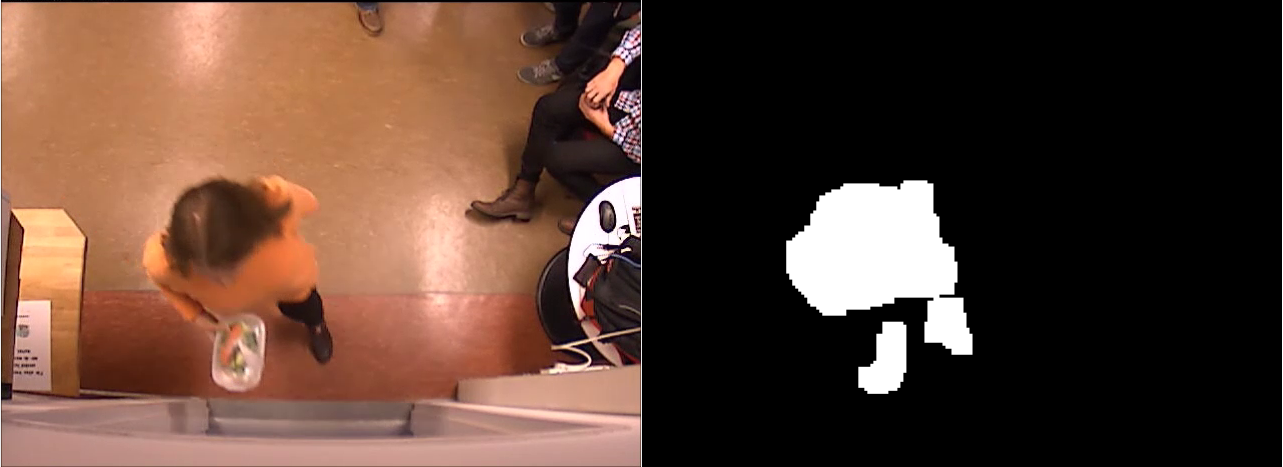
\includegraphics[width=\linewidth]{images/bg_success.png}
	\caption[An example of scattered binary mask of a human from the background model.]{\textit{The left image shows a moving person who is detected by the background subtractor. The right image shows the binary image generated from the left image, illustrating the scattered parts separated due to none-uniform motion.
	}}
	\label{fig:bg_success}  %Skapar referens till figuren
\end{figure}


\newpage

\section{An unsuccessful attempt - head detection by means of circle detection.}
\label{sec:hough_circles}

In \cite{Gardel} Gardel et.al. a method of head detection from above based on circle detection is proposed. In their approach circles, i.e. heads, are detected by first performing canny edge detection on each image frame and then performing a form of hough voting to detect circles. The hough voting is done by combining the results of a series of different filters designed to give high responses at circle and ellipse centers. We implemented their approach and experimented with many different variations of filter sizes and canny variables, with both types of circle filters described in the paper. We also tried using background subtraction on the canny image, using a mixture of Gaussian-based foreground segmentation \cite{Zivkovic} of the raw image, which gave slightly better results in simple situations. We were however not able to get any usable results for anything but the simplest cases, and therefore gave up on this approach after many fruitless attempts at tuning the system. Outputs from some of the different steps of cases where the approach was both successful and unsuccessful can be seen in figure \ref{fig:circle_success} and \ref{fig:circle_fail} below.
\vspace{1cm}
\begin{figure}[htb]
	\centering
	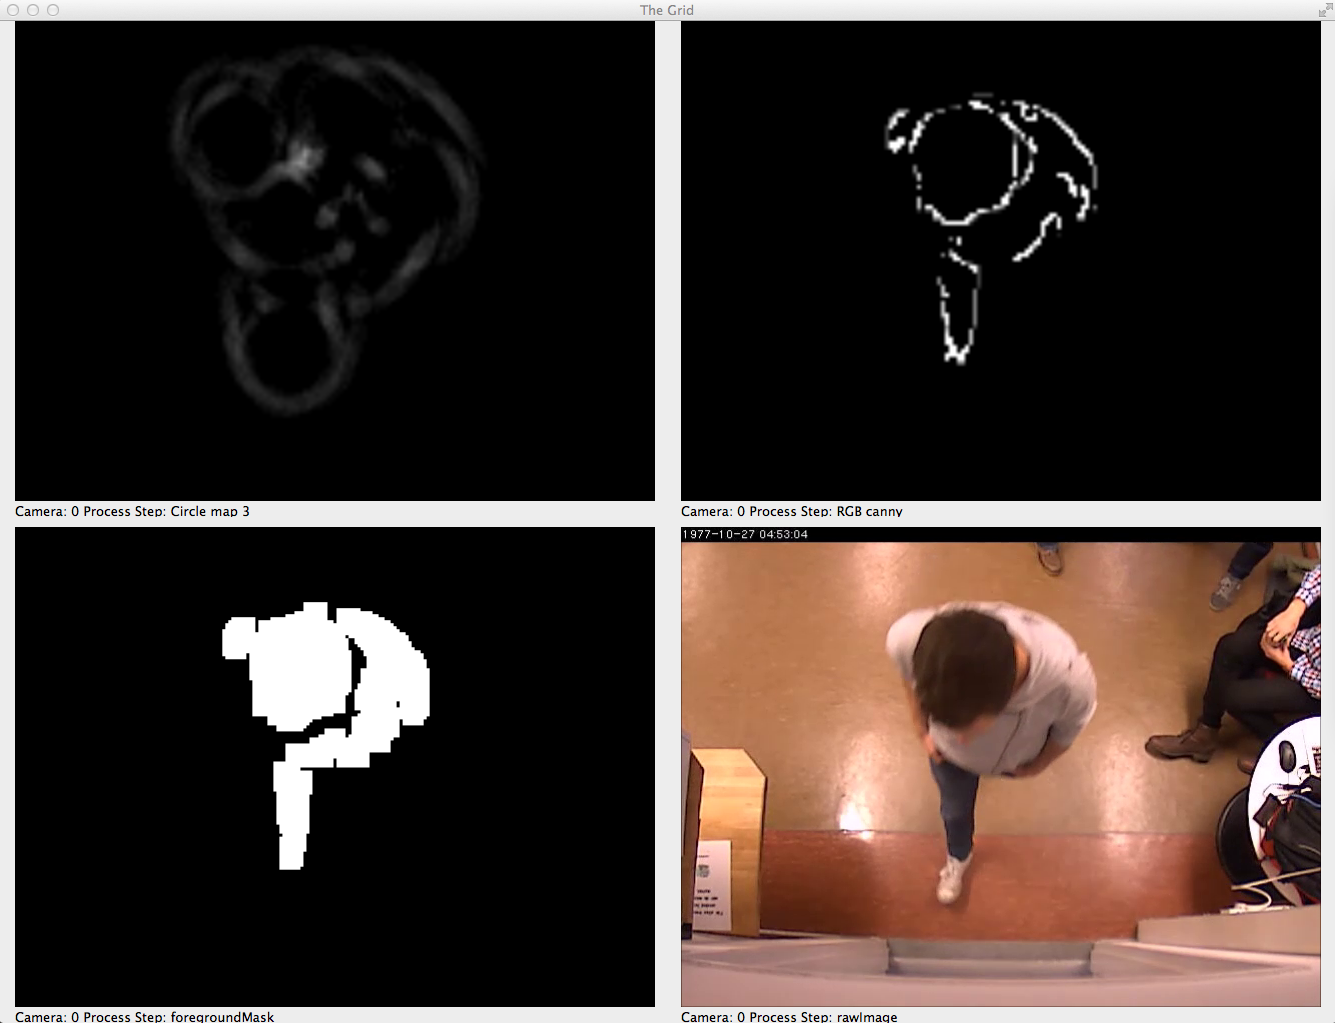
\includegraphics[width=\linewidth]{images/circle_detection_success.png}
	\caption[An example of a successful Hough-circle detection]{\\\textit{
	Top left: output from one of the circle filters.\\ 
	Top right: output from the canny edge detection after background subtraction.\\ 
	Bottom left: foreground mask.\\ 
	Bottom right: raw image.}}
	\label{fig:circle_success}  %Skapar referens till figuren
\end{figure}
\newpage
\begin{figure}[htb]
	\centering
	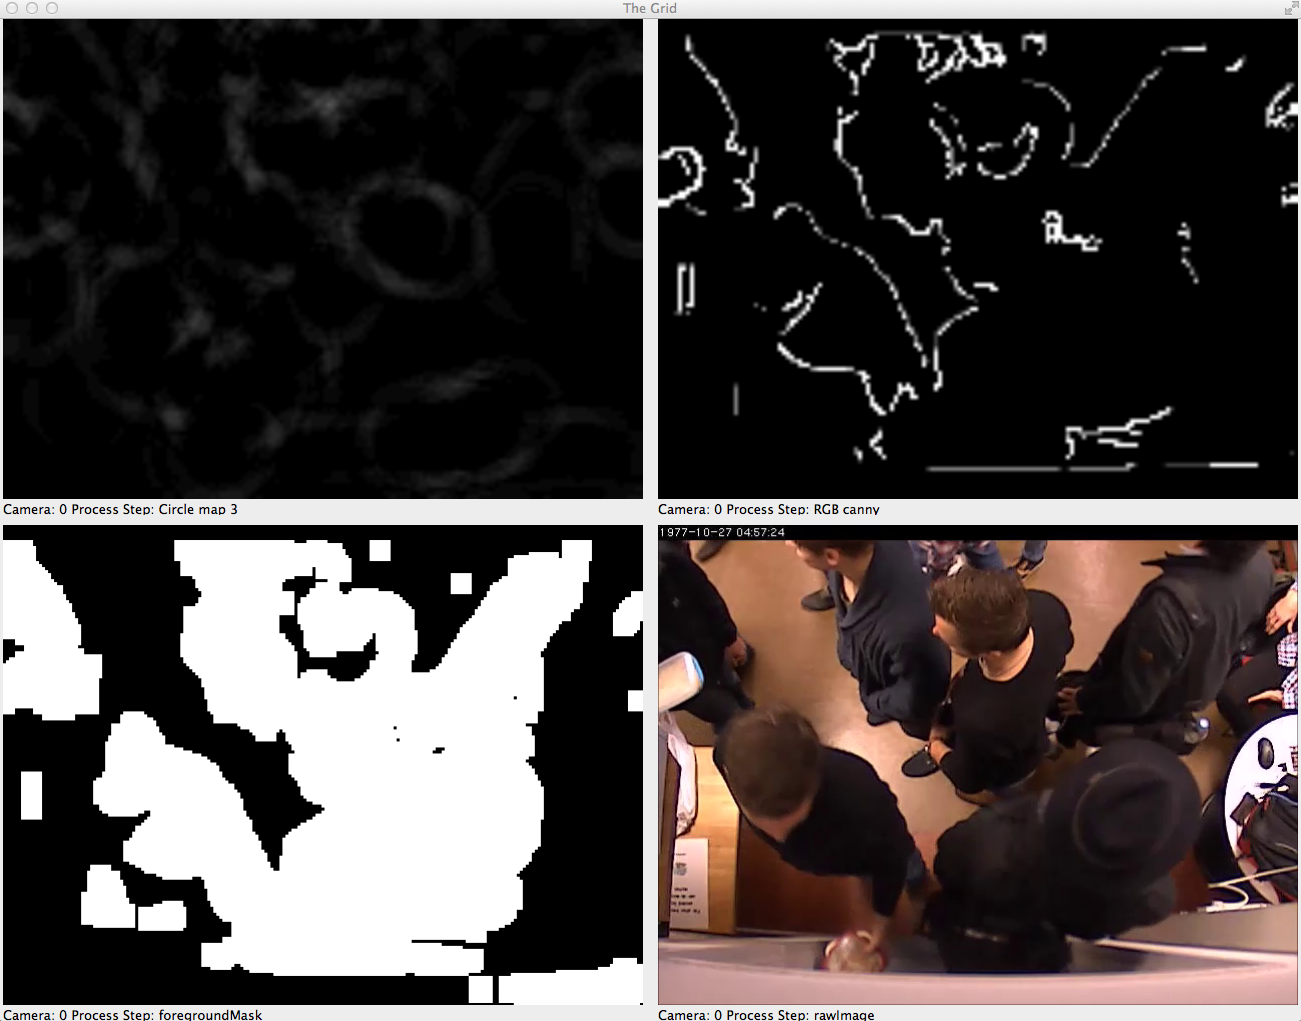
\includegraphics[width=\linewidth]{images/circle_detection_fail.png}
	\caption[An example of a failed Hough-circle detection]{\textit{\\
	Top left: output from one of the circle filters.\\
	Top right: output from the canny edge detection after background subtraction.\\
	Bottom left: foreground mask. \\
	Bottom right: raw image.}}
	\label{fig:circle_fail}  %Skapar referens till figuren
\end{figure}


\newpage

\section{Explored possibility - Depth image from stereo.}
\label{sec:stereoBM}

There are different ways in which one can obtain depth information. The easiest is perhaps to use a Kinect sensor which does all the job for you. However, this sensor is not compatible with the initially intended platform, namely the Raspberry Pi. An alternative to the Kinect is to use stereo vision. The semi-global stereo block matching algorithm proposed in \cite{StereoBM} was tested with partly successful results. The problem is its speed. Each frame takes approximately 300 ms to process which is too much for this application. This could be remedied to some extend by sacrificing image quality. The computation time can be reduced to 50 ms but the result is harder to use in later process steps. This algorithm could have been greatly sped up by a GPU implementation, but this approach was abandoned in favor for the Kinect which is both faster and easier to use. The results can be seen in figure \ref{fig:Stereo} below.

\vspace{1cm}
\begin{figure}[htb]
	\includegraphics[width=\linewidth]{images/stereoComp.png}
	\caption[An example of depth images calculated from a stereo sequence]{\textit{Evaluation of stereo block matching for depth calculations.\\ 
	Top: Left and right image of stereo sequence.\\ 
	Bottom left: Faster approach with lower quality.\\ 
	Bottom right: Slower approach with good quality.}}
	\label{fig:Stereo}  %Skapar referens till figuren
\end{figure}
\newpage


\newpage

%
% Bibliography
%

% Force a blank page so the bibliography starts on a new page.
% Comment out if not necessary
%\newpage
\thispagestyle{fancy}
\mbox{}
\begin{thebibliography}{9}
\addcontentsline{toc}{section}{References} % Add an entry for this in the table of contents

\bibitem{Gardel}
	Gardel, A., Bravo, I., Jimenez, P., Lazaro, J.L. \& Torquemada, A.\\
	``\textit{Statistical Background Models with Shadow Detection for Video Based Tracking},''\\ Intelligent Signal Processing, 2007. WISP 2007. IEEE International Symposium on?? Page: 1-6.
	
\bibitem{Zivkovic}
	Zivkovic, Z. \& Heijden, F.\\
	``\textit{Efficient Adaptive Density Estimation per Image Pixel for the Task of Background Subtraction},''\\
	Pattern recognition letters, Vol. 27, No. 7. (2006), pp. 773-780.

\vspace{2cm}
\LARGE{\textbf{EXAMPLE REFERENCES ONLY, REMOVE BEFORE HANDING IN}}
\normalsize
\bibitem{CVBook}
	Sonka, M., Hlavac, V. \& Boyle, R. 
	\emph{Image Processing, Analysis, and Machine Vision}.\\
	Toronto: Thompson Learning,
	cop. 2008, 3rd ed.,
	ISBN 0495244384.
	
\bibitem{Wood}
	Wood, J. (2007)
	``\textit{Statistical Background Models with Shadow Detection for Video Based Tracking},''\\
	Master thesis, Linköping University, Department of Electrical Engineering.	

\bibitem{DSPBook}
	Gustafsson, F., Ljung, L. \& Millnert, M.
	\emph{Signal Processing}.\\
	Studentlitteratur, Lund, Sweden,
	2011, 1st ed.,
	ISBN 978--91--44--05835--1.

\bibitem{MOTA}
	Bernardin, K. \& Stiefelhagen, R (2008)\\
	``\textit{Evaluating Multiple Object Tracking Performance: The CLEAR MOT Metrics},''\\
	Interactive Systems Lab, Institut für Theoretische Informatik,\\
	Universität Karlsruhe, 76131 Karlsruhe, Germany

\bibitem{CAVIAR}
	``\textit{CAVIAR: Context Aware Vision using Image-based Active Recognition},''\\
	EC Funded CAVIAR project/IST 2001 37540\\
	http://homepages.inf.ed.ac.uk/rbf/CAVIAR/
	

%\bibitem{somePaper}
%	Q. Lastname,
%	``Some article title,''
%	\emph{Some scientific journal},
%	vol.~1337, no.~1337,
%	pp.~666--1337,
%	month.~1337.

\end{thebibliography}



\end{document}
